%
% File acl2014.tex
%
% Contact: giovanni.colavizza@epfl.ch
%%
%% Based on the style files for ACL-2013, which were, in turn,
%% Based on the style files for ACL-2012, which were, in turn,
%% based on the style files for ACL-2011, which were, in turn, 
%% based on the style files for ACL-2010, which were, in turn, 
%% based on the style files for ACL-IJCNLP-2009, which were, in turn,
%% based on the style files for EACL-2009 and IJCNLP-2008...

%% Based on the style files for EACL 2006 by 
%%e.agirre@ehu.es or Sergi.Balari@uab.es
%% and that of ACL 08 by Joakim Nivre and Noah Smith

\documentclass[11pt]{article}
\usepackage{acl2014}
\usepackage{times}
\usepackage{url}
\usepackage{latexsym}
\usepackage{todonotes}
\usepackage[nameinlink]{cleveref}

%\setlength\titlebox{5cm}

% You can expand the titlebox if you need extra space
% to show all the authors. Please do not make the titlebox
% smaller than 5cm (the original size); we will check this
% in the camera-ready version and ask you to change it back.


\title{Gaining insight into the Amazon product network (temporary title)}

\author{Dario Pavllo \\
  {\tt dario.pavllo@epfl.ch} \\\And
  Second Author \\
  {\tt mattia.artinelli@epfl.ch} \\\And
Third Author \\
{\tt niccolo.sacchi@epfl.ch} \\}

\date{}

\begin{document}
\maketitle
\begin{abstract}
This project aims to find unobserved patterns and insights within the large offer of products on the Amazon website. To conduct our research, we devised an algorithm that builds a graph of such products, where articles with similar characteristics are clustered in an innovative manner. According to our research, these clusters are proven more accurate than the standard Amazon category aggregations, which are human-made and therefore prone to errors. In addition, biases in brands and descriptions are emphasised.

\end{abstract}

\section{Introduction}
\todo[inline]{The introduction should contain: 1 general (and not too technical) description of what we are doing (backgroud, justification), 2 related work and challenges, 3 focus of the project or added value, 4 outline of the report structure}
Buying from huge e-commerce websites such as \emph{Amazon} has many advantages, but paradoxically, users are often confused by the vast variety of products. Users may have a rough idea about the characteristics of the product they want to buy, and they often undergo the same process of comparing similar products. We aim to remove this redundancy and aid them in their purchases, suggesting the best or most popular products that correspond to their search. For instance, comparing smartphones or laptops may be difficult due to the wide price range and the required technical knowledge. \\ 
We also aim to identify patterns in the products. Do brands affect popularity and price of a product? Is it possible to identify the best producs among similar ones? 
The rest of the report is organised as follows: \Cref{sec:datastruct} briefly explains the dataset structure, \Cref{sec:datapreprocessing} and \Cref{sec:explodatanalysis} describe how we have preprocessed and explored the dataset, \Cref{sec:graphanalysis} reports how we have developed our research, and finally \Cref{sec:conclusion} reports conclusions.

\section{Dataset structure}
\label{sec:datastruct}
We have been provided with a dataset of Amazon products, which consists of two JSON files: 
\begin{itemize}
	\item \textit{metadata}: contains information related to the products, such as their unique ID (\textit{ASIN}), category, description, \textit{sales rank}, brand, price, and relations with other items. Such relations, which are of fundamental importance for building our graph, indicate how items are bought and visualized together. The size of the file is 9.81 GB (uncompressed).
	\item \textit{reviews}: contains ratings and reviews associated to each product, as well as the helpfulness of each review. The size of the file is approximately 87 GB (uncompressed).
\end{itemize}

\section{Dataset preprocessing}
\label{sec:datapreprocessing}
The dataset, due to its large size, could not be handled directly using Pandas. It has been processed using PySpark, first on the cluster (especially for \textit{reviews}) and then locally. While it may seem inappropriate at first, using Spark in local mode is indicated for medium-sized datasets (like the metadata one), as it automatically parallelizes jobs using all cores and spills to disk intermediate results that cannot fit in main memory. 

Since the text content of \textit{reviews} was not necessary for our  analysis, for each product, we extracted average rating, number of reviews, and their \textit{helpfulness} score. These fields have been then merged with \textit{metadata}.

We noticed that products were distributed over a wide set of categories, therefore, we decided to extract only the most relevant ones. We excluded categories in which purchase decision tends to depend more on people's personal preferences, rather than on an objective evaluation. Examples of such categories are \textit{Music}, \textit{Clothes} and \textit{Books}. We also decided to include only categories with a relatively large number of products. As a result, we created a with lighter dataset using only five categories:  \textit{Electronics}, \textit{Cell Phones \& Accessories}, \textit{Automotive}, \textit{Tools \& Home Improvement}, and \textit{Musical Instruments}. 

\section{Exploratory data analysis}
\label{sec:explodatanalysis}
We investigated what fields could exploited, analysing missing data, feature distributions and correlations.
\subsection{Missing data}
We observed that the quantity of missing entries significantly varies among the dataset fields. \textit{ASIN} and \textit{category} are always present by definition. In addition, almost all articles have at least one review. On the other hand, \textit{sales rank} and \textit{brand} are missing in about 60\% of cases. The remaining fields are overall present in the dataset, with a missing ratio lower than 30\%.
\subsection{Feature distribution}
\begin{figure}[h]
	\centering{}
	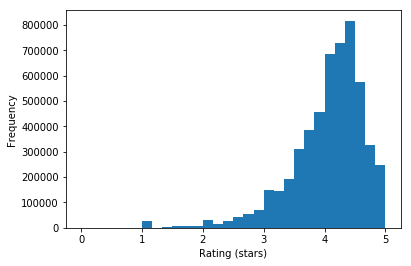
\includegraphics[width=0.47\textwidth]{img/avgReviews.png}
	\caption{Distribution of the \textit{average rating} field.}
	\label{fig:avgdist}
\end{figure}
\Cref{fig:avgdist} shows that ratings tend to be high. This evidence suggests that they may be not a good metric to evaluate the popularity of a product. The distribution of the number of reviews for each article is heavy-tailed (i.e. the mean is much larger than the median). Most reviews are regarded as helpful (50\% of the articles have an helpfulness percentage greater than 90\%), therefore, it is reasonable to consider them with good confidence.
\subsection{Correlation analysis}
We have investigated correlations among price, average rating and Sales rank. The analysis has been performed on whole dataset and not on the single categories independently. 
From Figure .... the correlation coefficients do not seem to be significant. However, some assumption could be asserted. As the price increases, the ratings tend to have lower variance and higher mean. In other words, more expensive products have averagegly higher ratings.
As the price increases, the sales rank tends to be lower (i.e. better). Costly products may be regarded as superior by people. 

\section{Graph analysis}
\label{sec:graphanalysis}
In order to analyse patterns and gain insights into the dataset, we have devised an algorithm to cluster products with similar characteristics, i.e. \textit{competing products}; however, without using directly any explicit characteristic (e.g. nor price nor average ratings). In particular, our first goal was to be able to numerically compare two products to decide which one is better. \todo{revise} We understood that before being able to compare two products, we had to cluster them in comparable products, as it would be meaningless to compare two products with very different characteristics (e.g. a cheap phone with a very expensive one). 

The algorithm builds a network of products using the relations between items provided in the dataset. In general terms, such relations have been collected by analysing the behaviour of Amazon's users, i.e. what products they buy or visualise together. We assumed that these relations could reflect meaningful patterns, as users tend to compare similar or related products.

\subsection{Graph structure}
The dataset has been transformed into graphs of relations between products, where vertices represent products, and edges represent competitions between products. To assure a coherent result and facilitate the computation, a graph includes only products of the same category. In details, we built the graph such that an edge from product A to product B is added if clients \textbf{buy} B after viewing A (\textit{buy after viewing} relation), but the edge between A and B is removed if A and B are frequently bought together (\textit{bought together} relation). The former means direct competition, i.e. an article has been preferred over another, while the latter means no competition, i.e. the two articles are complementary (e.g. a cellphone and a cover).

In previous experiments, we tried to build the graph by adding edges between products that are viewed together (\textit{also viewed} relation). This relation does not imply that any of the products has been actually bought, and it is produces a graph that is too dense to give meaningful results. Additionally, we believe that the also viewed relation is generated by Amazon's recommender system according to users' preferences, and it does not actually represent a graph relation. \todo{quote needed}

We could verify that the graph is sparse, which was also an important assumption. As a matter of fact, a fully connected graph would have produced spurious results that could be difficult to interpret. In addition, our analysis algorithms significantly benefit from a sparse graph, since they are NP-Complete. \todo{revise complexity}

We used the graph to analyse connected components, in particular max-cliques.
A max-clique is a set of totally interconnected nodes, which, in our scenario, represent products that are in direct competition among each other (and it is not really clear which one "wins"). Note that these competition relations might even comprehend products of the same brand: this could turn out to be an interesting tools for vendors.
\todo[inline]{should cliques and algorithm deserve more space here?}
\todo{connected components @ dario}
\todo{cartsimilarities @dario}


\subsection{Graph insights}
\todo[inline]{patterns (accumulators, cliques=competing products), prove that cliques represent competing products}
\todo[inline]{What do cliques represent? some of them are just same product with different colours, or same brand in clique}
We could observe that the graph is weakly connected. Most of the components have no relation among each other, and the average size of a component is small. The most important connected components are cliques, and we investigated if they effectively generated clusters of competing products. To validate our clusters, we have run the Boyer-Moore majority vote algorithm to prove that products in cliques belong to the same sub-category. \todo{check the price for validation?} As a result, we found that products are often incorrectly assigned to their category.

\subsection{Methodology}
Now that products are represented as nodes of a directed graph, a new feature becomes available: the product \textit{fan-in}, that is, how many incoming edges are associated to each node. Since an incoming edge indicates that a product has been preferred over another one, such new feature could be exploited to measure the popularity of a product. To prove it, we investigated correlations between fan-in and other features already included in the dataset, such as Sales rank, average rating, and number of reviews. 
\begin{figure}
	\centering{}
	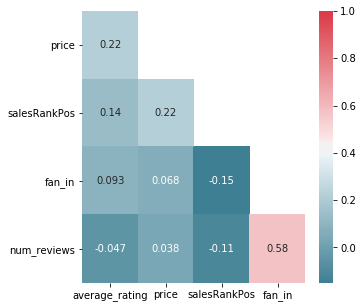
\includegraphics[width=0.5\textwidth]{img/faninCorr.png}
	\caption{Correlations between metrics.}
	\label{fig:faninCorr}
\end{figure}
As showed in \Cref{fig:faninCorr}, the fan-in has a moderate correlation with the number of reviews, and a weak correlation with the Sales rank. We also observed a weak correlation between the Sales rank and the price, which makes us suppose that people tend to prefer cheaper products. We can conclude that fan-in could be effectively used to measure the \textit{preference} of a product, i.e. how much the product is favoured over the others. In addition, fan-in shows several advantages over the other features. As mentioned in \Cref{sec:explodatanalysis}, Sales rank is present only in 60\% of the products. Moreover, it has a coarse granularity (i.e. it is computed almost only on macro-category), and it continuously evolves over time. \todo{quote needed}

\subsection{Predicting the best products}
We investigated how people decide what product is the best, analysing both textual and numerical features. In more formal terms, given two related products (e.g. the products in a cliques or in a graph relation), we predict the preferred one (i.e. the one with the highest fan-in) with of a binary classifier. In the \textit{learning to rank} context, such approach is known as the \textit{pairwise approach} \cite{Li:11}.
Textual features are extracted from the titles (with tf-idf vectorizer), as it represents a direct description of the product.
We subtract the feature vectors of the two products to produce the feature vector to supply to the classifier. As for the ground truth, provided that the subtraction is  A−BA−B , we put the label 0 if the winner is A, and 1 if the winner is B. For each sample, we also provide the opposite sample ( B−AB−A  with the inverted label), so that the classifier learns the commutative property and the classes are perfectly balanced.
We train a random forest on our data, with a fixed number of estimators (1000) and an optimal tree depth which is determined by grid search and cross-validation. Specifically, we perform a 5-fold cross-validation and select the depth that yields the best accuracy on the validation set.
We evaluate our model on a small test set (20\% of the data) to determine whether it overfitted or not.
We take the most important features learned by the random forest, and we try to interpret them. However, this is not sufficient, as we get only an indication of their magnitude (a positive value), and not whether they affect positively or negatively the result.
To get an idea of their impact, we select the top 1000 features (i.e. words) in terms of importance, and we use them to train a L2-regularized logistic regressor. By analyzing the weights learned by the latter, we can observe the sign of each feature, which corresponds to the impact (negative or positive) of the feature on the result.
While this process might seem convoluted, it is the result of many experiments. Initially, we tried to use L1-regularized logistic regression instead of random forests, which is expected to select only a few features (thanks to its sparsity property). Indeed, out of the thousands of features, only a few of them are selected. However, the model tends to overfit some features (e.g. the name of the model of a particular product, such as GT-I9500) in order to maximize the score, and these features are given a huge weight. As a result, it becomes impossible to interpret the model, as the useful features are buried by outliers.
On the other hand, random forests average the results of many weaks predictors, and are less susceptible to this kind of overfitting. Therefore, our idea is to use random forests to perform feature selection, and interpret the useful features using logistic regression.



\subsection{Bias in brands}
\todo[inline]{herding effect with number of reviews}

\section{Conclusion}
\label{sec:conclusion}

\todo[inline]{figures: 
rating distribution, 
correlations (between price, rating, salesrank,...) and with fan-in?, 
graph (cliques and accumulators),
decision boundaries classifier,
pairwise comparison/correlation}

%%%%%%%%%%%%%%%%%%%%%%%%%%%%% report ends here %%%%%%%%%%%%%%%%%%%%%%%%%%%%%%%%%%%

\clearpage
\newpage

%%%%%%%%%%%%%%%%%%%%%%  original document starts here %%%%%%%%%%%%%%%%%%%%%%%%%%%%


\section{Credits}

This document has been adapted from the instructions for earlier ACL
proceedings, including those for ACL-2012 by Maggie Li and Michael
White, those from ACL-2010 by Jing-Shing Chang and Philipp Koehn,
those for ACL-2008 by Johanna D. Moore, Simone Teufel, James Allan,
and Sadaoki Furui, those for ACL-2005 by Hwee Tou Ng and Kemal
Oflazer, those for ACL-2002 by Eugene Charniak and Dekang Lin, and
earlier ACL and EACL formats. Those versions were written by several
people, including John Chen, Henry S. Thompson and Donald
Walker. Additional elements were taken from the formatting
instructions of the {\em International Joint Conference on Artificial
  Intelligence}.

\section{Introduction}

The following instructions are directed to the ADA students who decided to prepare a report. Authors are
required to provide a Portable Document Format (PDF) version of their
reports. It must be maximum 4-page long, excluding references.

\section{General Instructions}

Manuscripts must be in two-column format.  Exceptions to the
two-column format include the title, authors' names and complete
addresses, which must be centered at the top of the first page, and
any full-width figures or tables (see the guidelines in
Subsection~\ref{ssec:first}). {\bf Type single-spaced.}  Start all
pages directly under the top margin. See the guidelines later
regarding formatting the first page.

\subsection{Format of Electronic Manuscript}
\label{sect:pdf}

For the production of the electronic manuscript you must use Adobe's
Portable Document Format (PDF). PDF files are usually produced from
\LaTeX\ using the \textit{pdflatex} command. If your version of
\LaTeX\ produces Postscript files, you can convert these into PDF
using \textit{ps2pdf} or \textit{dvipdf}. On Windows, you can also use
Adobe Distiller to generate PDF.

Please make sure that your PDF file includes all the necessary fonts
(especially tree diagrams, symbols, and fonts with Asian
characters). When you print or create the PDF file, there is usually
an option in your printer setup to include none, all or just
non-standard fonts.  Please make sure that you select the option of
including ALL the fonts. \textbf{Before sending it, test your PDF by
  printing it from a computer different from the one where it was
  created.} Moreover, some word processors may generate very large PDF
files, where each page is rendered as an image. Such images may
reproduce poorly. In this case, try alternative ways to obtain the
PDF. One way on some systems is to install a driver for a postscript
printer, send your document to the printer specifying ``Output to a
file'', then convert the file to PDF.

It is of utmost importance to specify the \textbf{A4 format} (21 cm
x 29.7 cm) when formatting the report. When working with
{\tt dvips}, for instance, one should specify {\tt -t a4}.

Print-outs of the PDF file on A4 report should be identical to the
hardcopy version.


\subsection{Layout}
\label{ssec:layout}

Format manuscripts two columns to a page, in the manner these
instructions are formatted. The exact dimensions for a page on A4
report are:

\begin{itemize}
\item Left and right margins: 2.5 cm
\item Top margin: 2.5 cm
\item Bottom margin: 2.5 cm
\item Column width: 7.7 cm
\item Column height: 24.7 cm
\item Gap between columns: 0.6 cm
\end{itemize}

\noindent Papers should not be submitted on any other report size, no exceptions.


\subsection{Fonts}

For reasons of uniformity, Adobe's {\bf Times Roman} font should be
used. In \LaTeX2e{} this is accomplished by putting

\begin{quote}
\begin{verbatim}
\usepackage{times}
\usepackage{latexsym}
\end{verbatim}
\end{quote}
in the preamble. If Times Roman is unavailable, use {\bf Computer
  Modern Roman} (\LaTeX2e{}'s default).  Note that the latter is about
  10\% less dense than Adobe's Times Roman font.


\begin{table}[h]
\begin{center}
\begin{tabular}{|l|rl|}
\hline \bf Type of Text & \bf Font Size & \bf Style \\ \hline
report title & 15 pt & bold \\
author names & 12 pt & bold \\
the word ``Abstract'' & 12 pt & bold \\
section titles & 12 pt & bold \\
document text & 11 pt  &\\
captions & 11 pt & \\
abstract text & 10 pt & \\
bibliography & 10 pt & \\
footnotes & 9 pt & \\
\hline
\end{tabular}
\end{center}
\caption{\label{font-table} Font guide.}
\end{table}

\subsection{The First Page}
\label{ssec:first}

Center the title and author's name(s) across both
columns. Do not use footnotes for affiliations. Use the
two-column format only when you begin the abstract.

{\bf Title}: Place the title centered at the top of the first page, in
a 15-point bold font. (For a complete guide to font sizes and styles,
see Table~\ref{font-table}) Long titles should be typed on two lines
without a blank line intervening. Approximately, put the title at 2.5
cm from the top of the page, followed by a blank line, then the
author's names(s) on the following line. Do not
use only initials for given names (middle initials are allowed). Do
not format surnames in all capitals (e.g., use ``Schlangen'' not
``SCHLANGEN'').  Do not format title and section headings in all
capitals as well except for proper names (such as ``BLEU'') that are
conventionally in all capitals. Start the body of the first page 7.5 cm from the top of the
page.

{\bf Abstract}: Type the abstract at the beginning of the first
column. The width of the abstract text should be smaller than the
width of the columns for the text in the body of the report by about
0.6 cm on each side. Center the word {\bf Abstract} in a 12 point bold
font above the body of the abstract. The abstract should be a concise
summary of the general thesis and conclusions of the report. It should
be no longer than 150 words. The abstract text should be in 10 point font.

{\bf Text}: Begin typing the main body of the text immediately after
the abstract, observing the two-column format as shown in 
the present document. Do not include page numbers.

{\bf Indent} when starting a new paragraph. Use 11 points for text and 
subsection headings, 12 points for section headings and 15 points for
the title. 

\subsection{Sections}

{\bf Headings}: Type and label section and subsection headings in the
style shown on the present document.  Use numbered sections (Arabic
numerals) in order to facilitate cross references. Number subsections
with the section number and the subsection number separated by a dot,
in Arabic numerals. Do not number subsubsections.

{\bf Citations}: Citations within the text appear in parentheses
as~\cite{Gusfield:97} or, if the author's name appears in the text
itself, as Gusfield~\shortcite{Gusfield:97}.  Append lowercase letters
to the year in cases of ambiguity.  Treat double authors as
in~\cite{Aho:72}, but write as in~\cite{Chandra:81} when more than two
authors are involved. Collapse multiple citations as
in~\cite{Gusfield:97,Aho:72}. Also refrain from using full citations
as sentence constituents. We suggest that instead of
\begin{quote}
  ``\cite{Gusfield:97} showed that ...''
\end{quote}
you use
\begin{quote}
``Gusfield \shortcite{Gusfield:97}   showed that ...''
\end{quote}

If you are using the provided \LaTeX{} and Bib\TeX{} style files, you
can use the command \verb|\newcite| to get ``author (year)'' citations.

\textbf{Please do not use anonymous citations} and do not include
acknowledgements when submitting your reports..

\textbf{References}: Gather the full set of references together under
the heading {\bf References}. Arrange the references alphabetically
by first author, rather than by order of occurrence in the text.
Provide as complete a citation as possible, using a consistent format,
such as the one for {\em Computational Linguistics\/} or the one in the 
{\em Publication Manual of the American 
Psychological Association\/}~\cite{APA:83}.  Use of full names for
authors rather than initials is preferred.  A list of abbreviations
for common computer science journals can be found in the ACM 
{\em Computing Reviews\/}~\cite{ACM:83}.

\subsection{Footnotes}

{\bf Footnotes}: Put footnotes at the bottom of the page and use 9
points text. They may be numbered or referred to by asterisks or other
symbols.\footnote{This is how a footnote should appear.} Footnotes
should be separated from the text by a line.\footnote{Note the line
separating the footnotes from the text.}

\subsection{Graphics}

{\bf Illustrations}: Place figures, tables, and photographs in the
report near where they are first discussed, rather than at the end, if
possible.  Wide illustrations may run across both columns.

{\bf Captions}: Provide a caption for every illustration; number each one
sequentially in the form:  ``Figure 1. Caption of the Figure.'' ``Table 1.
Caption of the Table.''  Type the captions of the figures and 
tables below the body, using 11 point text.

\begin{thebibliography}{}

\bibitem[\protect\citename{Amazon:bestsell}]{Amazon:bestsell}
Amazon.
\newblock {\em About Amazon Best Sellers Rank.}

\bibitem[\protect\citename{Li}2011]{Li:11}
Hang Li.
\newblock 2011.
\newblock {\em A Short Introduction to Learning to Rank.}

\bibitem[\protect\citename{Aho and Ullman}1972]{Aho:72}
Alfred~V. Aho and Jeffrey~D. Ullman.
\newblock 1972.
\newblock {\em The Theory of Parsing, Translation and Compiling}, volume~1.
\newblock Prentice-{Hall}, Englewood Cliffs, NJ.

\bibitem[\protect\citename{{American Psychological Association}}1983]{APA:83}
{American Psychological Association}.
\newblock 1983.
\newblock {\em Publications Manual}.
\newblock American Psychological Association, Washington, DC.

\bibitem[\protect\citename{{Association for Computing Machinery}}1983]{ACM:83}
{Association for Computing Machinery}.
\newblock 1983.
\newblock {\em Computing Reviews}, 24(11):503--512.

\bibitem[\protect\citename{Chandra \bgroup et al.\egroup }1981]{Chandra:81}
Ashok~K. Chandra, Dexter~C. Kozen, and Larry~J. Stockmeyer.
\newblock 1981.
\newblock Alternation.
\newblock {\em Journal of the Association for Computing Machinery},
  28(1):114--133.

\bibitem[\protect\citename{Gusfield}1997]{Gusfield:97}
Dan Gusfield.
\newblock 1997.
\newblock {\em Algorithms on Strings, Trees and Sequences}.
\newblock Cambridge University Press, Cambridge, UK.

\end{thebibliography}

\end{document}
